\documentclass{beamer}
\usetheme{Madrid}
\beamertemplatenavigationsymbolsempty
\setbeamertemplate{headline}{}
\setbeamertemplate{footline}[frame number]
\AtBeginEnvironment{frame}{\raggedright}
\usepackage{pgfplots}
\pgfplotsset{compat=1.17}
\title{Regresi\'on Log\'istica para Clasificaci\'on de Ventanas}
\author{Nota T\'ecnica Interna}
\date{\today}

\begin{document}

\begin{frame}{Motivaci\'on: Decisiones Probabil\'isticas}
\begin{itemize}
    \item Etiqueta binaria con probabilidad \(p(y=1\mid x)\), no solo clase dura.
    \item Puntaje \(z=b+w^\top x\) es no acotado; se enlaza a \([0,1]\).
    \item \textbf{Puntaje vs probabilidad}: \(z\) solo ordena; \(\sigma(z)\) es calibrada.
    \item Ejemplo: \(z=0.2\Rightarrow p\approx0.55\); \(z=-2\Rightarrow p\approx0.12\).
\end{itemize}
\end{frame}

\begin{frame}{Enlace Sigmoide y Geometr\'ia}
\begin{itemize}
    \item Sigmoide: \(\sigma(z)=\tfrac{1}{1+e^{-z}}\) comprime cualquier puntaje a \([0,1]\).
    \item \(z=b+w^\top x\) es distancia con signo al hiperplano (escalada por \(\lVert w\rVert\)).
    \item La pendiente es m\'axima en \(z=0\); cerca de la frontera hay mayor incertidumbre.
    \item Mini chequeo: \(x=(1,2), w=(0.3,0.4), b=-0.5\Rightarrow z=0.6, p\approx0.65\).
\end{itemize}
\begin{center}
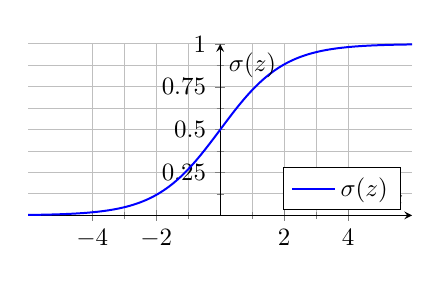
\begin{tikzpicture}[scale=0.9]
\begin{axis}[
    width=7cm, height=4cm,
    axis lines=middle,
    xlabel={$z$}, ylabel={$\sigma(z)$},
    xmin=-6, xmax=6, ymin=0, ymax=1,
    samples=200, domain=-6:6, grid=both, minor tick num=1,
    xtick={-4,-2,0,2,4}, ytick={0,0.25,0.5,0.75,1},
    legend pos=south east, legend cell align=left
]
\addplot[blue, thick] {1/(1+exp(-x))};
\legend{$\sigma(z)$}
\end{axis}
\end{tikzpicture}
\end{center}
\end{frame}

\begin{frame}{Log-Odds Lineales}
\begin{itemize}
    \item Transformaci\'on logit: \(\log \tfrac{p}{1-p} = b + w^\top x\).
    \item Logit af\'in en \(x\) \(\Rightarrow\) frontera \(w^\top x + b = 0\) es un hiperplano (modelo lineal).
    \item Monoton\'ia: ordenar por \(z\) o por \(p\) es equivalente.
\end{itemize}
\end{frame}

\begin{frame}{Verosimilitud Bernoulli}
\begin{itemize}
    \item Para datos i.i.d., \(p_i = \sigma(b + w^\top x_i)\).
    \item Verosimilitud: \[\mathcal{L}(w,b)=\prod_i p_i^{y_i}(1-p_i)^{(1-y_i)}.\]
    \item Maximizar \(\mathcal{L}\) elige \(w,b\) que hacen m\'as probables las etiquetas observadas.
\end{itemize}
\end{frame}

\begin{frame}{MLE y P\'erdida Logar\'itmica}
\begin{itemize}
    \item Log-verosimilitud negativa: \[\text{NLL}=-\sum_i \big[y_i\log(p_i)+(1-y_i)\log(1-p_i)\big].\]
    \item Minimizar NLL equivale a minimizar cross-entropy binaria (log-loss).
    \item Lectura: los errores confiados se penalizan fuertemente; los inciertos, menos.
\end{itemize}
\end{frame}

\begin{frame}{Regularizaci\'on (L2)}
\begin{itemize}
    \item Se agrega \(\lambda\lVert w\rVert^2\) a la NLL para limitar pesos grandes.
    \item Vista geom\'etrica: L2 mantiene \(w\) dentro de una hiperesfera; penaliza por igual en todas las direcciones.
    \item Reduce sobreajuste y estabiliza caracter\'isticas correlacionadas.
    \item En scikit-learn, `C` es inverso de la fuerza: \(\lambda = \tfrac{1}{2C}\); `C` menor $\Rightarrow$ m\'as shrinkage.
\end{itemize}
\begin{center}
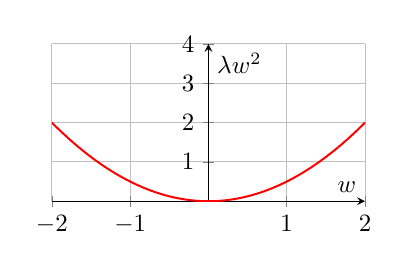
\begin{tikzpicture}[scale=0.9]
\begin{axis}[
    width=6cm, height=3.8cm,
    axis lines=middle,
    xlabel={$w$}, ylabel={$ \lambda w^2$},
    xmin=-2, xmax=2, ymin=0, ymax=4,
    samples=200, domain=-2:2, grid=major, minor tick num=0,
    xtick={-2,-1,0,1,2}, ytick={0,1,2,3,4},
]
\addplot[red, thick] {0.5*x^2};
\end{axis}
\end{tikzpicture}
\end{center}
\end{frame}

\begin{frame}{Desbalance de Clases}
\begin{itemize}
    \item `class\_weight="balanced"` define peso para clase \(c\): \(\text{peso}_c = \tfrac{N}{2N_c}\) (inversa de frecuencia).
    \item Cada t\'ermino de p\'erdida se multiplica por su peso, dando m\'as impacto a errores en la minor\'ia.
    \item Ayuda a alinear umbral efectivo con recall/precision cuando los positivos son raros.
\end{itemize}
\end{frame}

\begin{frame}{Predicci\'on, Umbral, Ranking}
\begin{itemize}
    \item `predict\_proba` entrega \(p = \sigma(b + w^\top x)\); decisi\'on por defecto usa 0.5.
    \item Bajar el umbral reduce FN pero sube FP; subirlo hace lo contrario.
    \item ROC AUC eval\'ua el ranking por \(p\) (o \(z\)) sin fijar umbral.
    \item Mini diagrama: features \(\rightarrow z=b+w\cdot x \rightarrow \sigma(z) \rightarrow p \rightarrow\) umbral \(\rightarrow\) clase.
\end{itemize}
\begin{center}
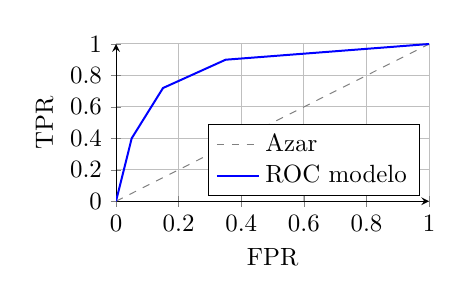
\begin{tikzpicture}[scale=0.9]
\begin{axis}[
    width=6cm, height=3.8cm,
    axis lines=left,
    xlabel={FPR}, ylabel={TPR},
    xmin=0, xmax=1, ymin=0, ymax=1,
    grid=major, legend pos=south east, legend cell align=left
]
\addplot[gray, dashed] coordinates {(0,0) (1,1)};
\addplot[blue, thick] coordinates {(0,0) (0.05,0.4) (0.15,0.72) (0.35,0.9) (1,1)};
\legend{Azar,ROC modelo}
\end{axis}
\end{tikzpicture}
\end{center}
\end{frame}

\end{document}
